%\documentclass[margin=0mm]{standalone}
%\usepackage{tikz}
%\usepackage{pgfplots}
% \pgfplotsset{compat=newest}
%
%
%\usepackage{currfile,hyperxmp}
%\usetikzlibrary{math,matrix,fit,positioning}
%\usepgfplotslibrary{groupplots}
%
%
%\begin{document}

  

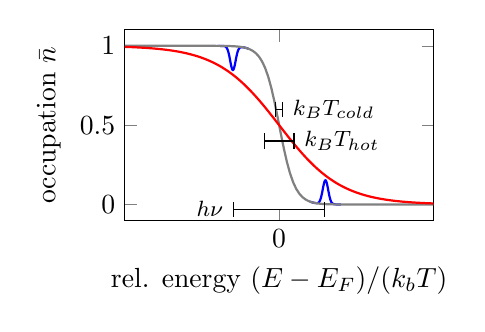
\begin{tikzpicture}
%\useasboundingbox (-1.0,-1.0) rectangle (10.2,4.2);
%\draw (-1,-1.0) rectangle (10.2,4.2);
%

 
\begin{axis}[width=55mm, height=40mm, ylabel = {occupation $\bar{n}$}, xlabel = {rel. energy  $(E - E_F) / (k_b T)$},
%[ytick = \empty, yticklabel = \empty,
%ylabel = {extinktion}, xlabel = {energy (eV)},
%ytick pos = left, 
xtick = {0}, 
 xmin=-20, xmax = 20,
 ]
\
\addplot[blue,thick, domain= -4:-8, samples=100]{ 1/ (exp(x) + 1)  - 0.15* exp(- (x+6)^2 / 0.25) };
\addplot[blue, thick,domain= 4:8, samples=100]{   1/ (exp(x) + 1)  +  0.15* exp(- (x-6)^2 / 0.25)) };
\addplot[gray, thick, domain=-20:20, samples=100]{1 / (exp(x) + 1)};

\addplot[red, thick,domain=-20:20, samples=100]{1 / (exp(x/4) + 1)};

\draw[|-|] (-0.5, 0.6) -- (0.5, 0.6) node[right] {\footnotesize $k_B T_{cold}$};
\draw[|-|] (-2, 0.4) -- (2, 0.4) node[right] {\footnotesize $k_B T_{hot}$};

\draw[|-|] (-6, -0.03) node[left] {\footnotesize $h \nu$} -- (6, -0.03) ;

\end{axis}


\end{tikzpicture}

%\end{document}